\section{Results}

\subsection{Article-Editor Ranking Calibration}

Having our endogenous and exogenous variables now, we perform tests to
$\underset{\alpha, \beta}{\operatorname{argmax}} \rho(\alpha, \beta)$, the pair that maximizes our spearman rank correlation between  $\mathbf{w^{*}_{e}}$ and $v_e$. We also do so for $\mathbf{w^{*}_{a}}$ and $v_a$.

First we used a general purpose maximizing algorithm to find maximizing values. Secondly we performed a grid search with visual inspection. Overall we find smooth landscapes. The two methods verified each other's results. \ref{fig:contour_fem} shows the correlation landscape for Category:Feminist Writers calibrating both articles and editors.

The results of calibrating our model are encouraging as we find high correlations between the results of our $w^*_e$ algorithm and our exogenous variables $v$. 

We define $\rho$ at the maximum achievable spearman rank correlation between $w^*$ and $v$ for editors or articles, by category, and over time. The variation of $\rho$, by for editor for any category ranges from 0.75 to 0.46 with a mean 0.64.  That same statistic for articles is articles from 0.91 to 0.57 with a mean of 0.72, which is overall higher.

 
From snapshotting we see view $\rho$ as  a function of time. In the case of editors we see increasing trends in all categories over time in an asymptotic way. This means that $w^*_e$ benefits from incorporating more contribution history. That is, as a category matures we can better predict successful editors from which articles they edit. As for being able to predict article quality, from the start of a category's history the correlations remain high and  stable. It is easier to predict an articles quality based on who has edited it.  \ref{fig:rhotime}

\begin{figure}[!t]
\centering
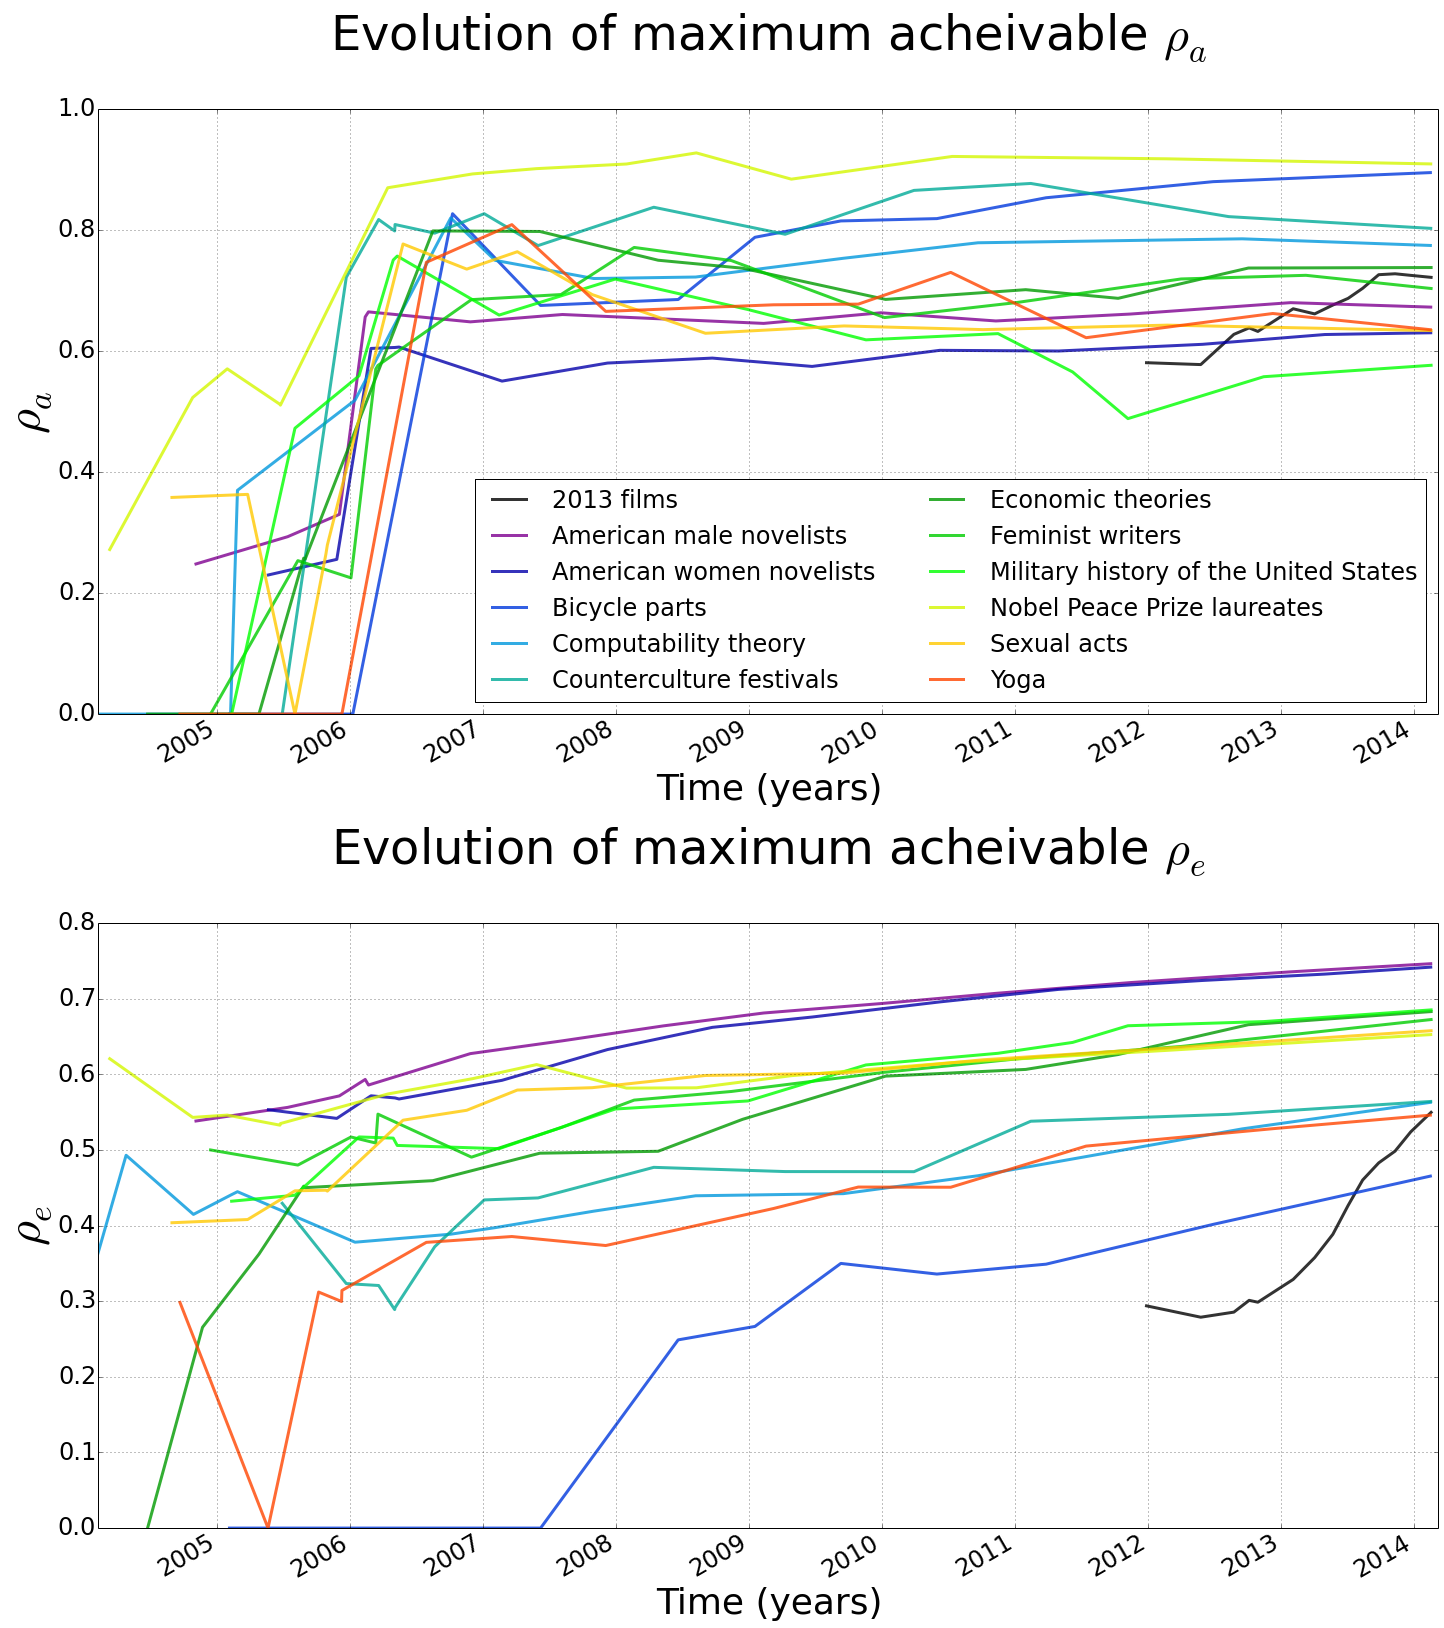
\includegraphics[width=0.9\columnwidth]{Figures/rho_combined.png}.
\caption{$\rho$ over time, by category and type}
\label{fig:rhotime}
\end{figure}


\subsection{Negative values of $\alpha$ and $\beta$}
Another surprising result is that we find at times, negative values for $\alpha$ and $\beta$.

To understand the results, we must have a firm grasp on what $\alpha$ and $\beta$ mean. They are more easily understood by roughly rewriting $\mathbf{w^*}$ as:
\begin{equation}
\begin{cases}
w^{*}_{e} \sim k^{1-\beta}_{e} \langle k_{a}^{-\alpha}\rangle_e \\
w^{*}_{a} \sim k^{1-\alpha}_{a} \langle k_{e}^{-\beta}\rangle_a
\end{cases} \label{eqsim}
\end{equation}

Our solution spaces are not single point but a 2-dimensional area, similar to what found in \cite{caldarelli2012network}. A reason for this is the fact that we are using the spearman ranking correlation, once a ranking is achieved, $\alpha$ and $\beta$ can perturb without adjusting the ranking. 

In these areas we see trends in there being important axes shown by the maximizing segments, which represent a several explanations for the article behaviour behaviour.

With regards to \eqref{eqsim}, we can see the similarity of $w^*$ is related to the product of two expression. Values of $\alpha$ and $\beta$ can make the one of the product approach one or and so the other parameter may dominate. In the article plot of \ref{fig:contour_fem} our solution spaces moves linearly from $0 <\alpha <1 , \beta \approx 0$ meaning that successful editors are charcterized, by an equal balance of their edit count, and the average article quality of articles they've edited. At the other end $\alpha < - 1 , \beta > 1$ anti-importance of their how man articles they've edited, but high importance on the quality of edits.

This seems quite natural to say, but $\alpha$ and $\beta$ need not vary together at all, and could be in different quadrants of the landscape each describing a different success strategy.

\begin{figure}[!t]
\centering
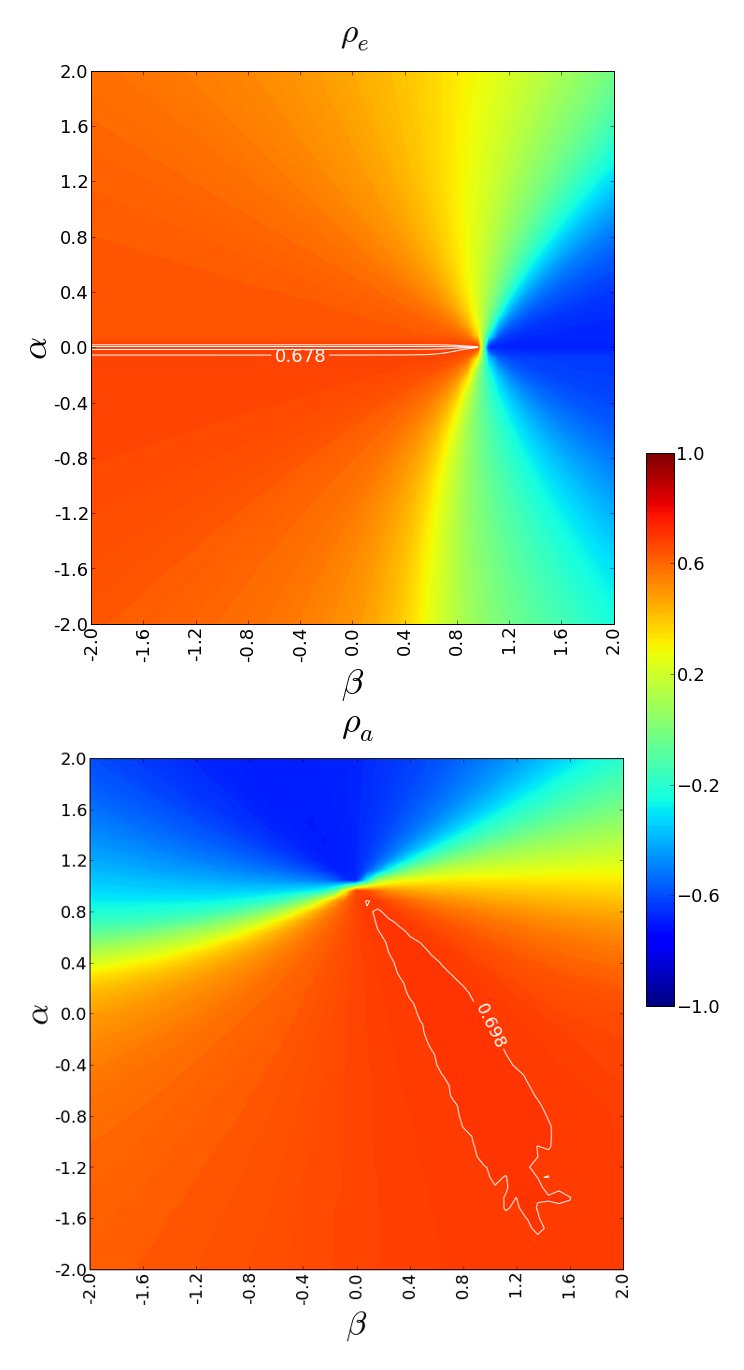
\includegraphics[width=0.9\columnwidth]{Figures/contour_fem_combined.png}.
\caption{Heatmaps of Spearman Rank Correlation between endogenous and exogenous ranks, 95$^{th}$ percentile  of correlations circled
Upper panel: articles - $w^*_a ~ v_a$
Lower panel editors - $w^*_e ~ v_e$
White indicates that correlation was not significant $p<0.05$ } 
\label{fig:contour_fem}
\end{figure}

\subsection{$\rho$ increases over time.}

	



